\newpage
\subsection{Долгосрочное планирование продаж}
\label{bp:monthplan}


Долгосрочным планированием продаж на ПРЕДПРИЯТИИ занимается ООО ТД ''ФОРМАТ''. %заместитель коммерческого директора.
ПРЕДПРИЯТИЕ входит в группу предприятий ''Объединенные бумажные фабрики'', далее по тексту ГП ''ОБФ'' .
Процесс долгосрочного планирования продаж происходит в соответствии с процессами описанными ниже.


  \textbf{Долгосрочное планирование - ''Стратегический план развития на 7 лет''}
    
Формируется стратегический план развития ГП ''ОБФ'' на 7 лет с указанием направлений развития ГП ''ОБФ'', таких как:  постановка новых целей, увеличение объема продаж, модернизация/покупка оборудования и т.д.

  \textbf{Среднесрочное планирование - ''Тактический план развития на 3 года''}
    
Тактическое планирование осуществляется согласно промежуточным стратегическим целям. Включает в себя планы действий и методы реализации стратегии, необходимые для формирования условий деятельности как ГП ''ОБФ'' в целом, так и отдельно каждого предприятия в составе группы.

\textbf{Краткосрочное планирование - ''Оперативный план развития на 1 год''}

Основные задачи краткосрочного планирования: достижение оперативных целей, решение текущих задач ГП ''ОБФ'' и ее структурных подразделений. Планирование предполагает оптимизацию используемых ресурсов. В оперативном планировании учитывается реальное состояние внешней и внутренней среды каждого предприятия в составе ГП ''ОБФ'' в планируемом периоде.
Формирование оперативного плана осуществляет планово-экономическим отдел.  
Внутри ГП ''ОБФ'' для обозначения оперативного плана именуется используется термин ''ПРОФИНТЕХПЛАН'' (форма \ref{pic:XI.1}).

Планово-экономический отдел производит расчет загрузки производственных мощностей по каждой единице оборудования с учетом графика работы предприятия, графика работы персонала, графика проведения ТО и ППР (рис. \ref{pic:XII.1.jpg}), а также норм времени (расчетная и фактическая, получаемая на основании статистических данных за прошедший год). Расчет загрузки производственных мощностей представлен на рис. \ref{pic:XI.12.jpg}.
Нормы выработки по каждой единице оборудования утверждаются один раз в год (рис. \ref{pic:XI.11..jpg}) и (рис. \ref{pic:XI.11.jpg}).

Плановая производственная мощность формируются на основании таких параметров как ''Часовая производственная мощность'' и ''Среднесуточная производственная мощность'', измеряемые в квадратных метрах и штуках.

%Расчетная производственная мощность = Плану производства = План продаж  = План реализации.


\textbf{Краткосрочное планирование - ''План продаж на 1 месяц''}

План продаж на 1 месяц формируется на базе статистических данных за последние 1,5 месяца. При изменении норм в расчет принимаются статистические данные собранные с момента введения новых норм, но не более 1,5 месяца.

Ежемесячно менеджеры отдела продаж в период с 20 по 24 число каждого месяца формируют отчет ''Ассортиментный план'' (рис. \ref{pic:I.5.6..jpg}), на основании которого рассчитываются и формируются плановые потребности на предстоящий месяц в разрезе марок картона, типов изделий, контрагентов.

Отчет ''Ассортиментный план'' формируется автоматически в системе 1С: УПП (рис. \ref{pic:I.5.6.jpg})
Менеджер вносит данные о планируемом количестве шт/м2 отдельно по каждой производственной линии, указывая действующую ТК.
Ассортиментный план корректируется и согласуется коммерческой отделом ООО ТД ''ФОРМАТ''. Ассортиментный план нужен для руководства и для краткосрочного планирования сырья.



%Долгосрочное (месячное) планирование продаж выполняется в отделе продаж (форма \ref{pic:d3}).
%До 25 числа каждого месяца каждый менеджер создает по своим заказчикам план продаж на будущий месяц по номенклатуре изделий и в количественном выражении. 
%План нужен для руководства и для долгосрочного планирования сырья.

%Коммерческий директор контролирует выполнение  плана продаж по отчету ''План продаж'' (рис. \ref{pic:d3}).
% Каждый понедельник все менеджеры формируют в таблице MS Excel план поступления денежных средств для коммерческого директора.





%Менеджеры ведут месячный план продаж в формате MS Excel.
%%План формируется стоимостных (тыс. руб.) показателях.
%Форма плана приведена на рис. \ref{pic:monthplan}.  

%Годовой план продаж разрабатывается коммерческим директором ООО ''ТД «Брянский картон'' и является целевым показателем для других подразделений производства (рис. \ref{pic:monthplan}).
%План является необходимым ограничением для менеджеров отдела продаж на год. План формируется в стоимостных (тыс. руб.) показателях.
% 
\begin{figure}
\begin{center}
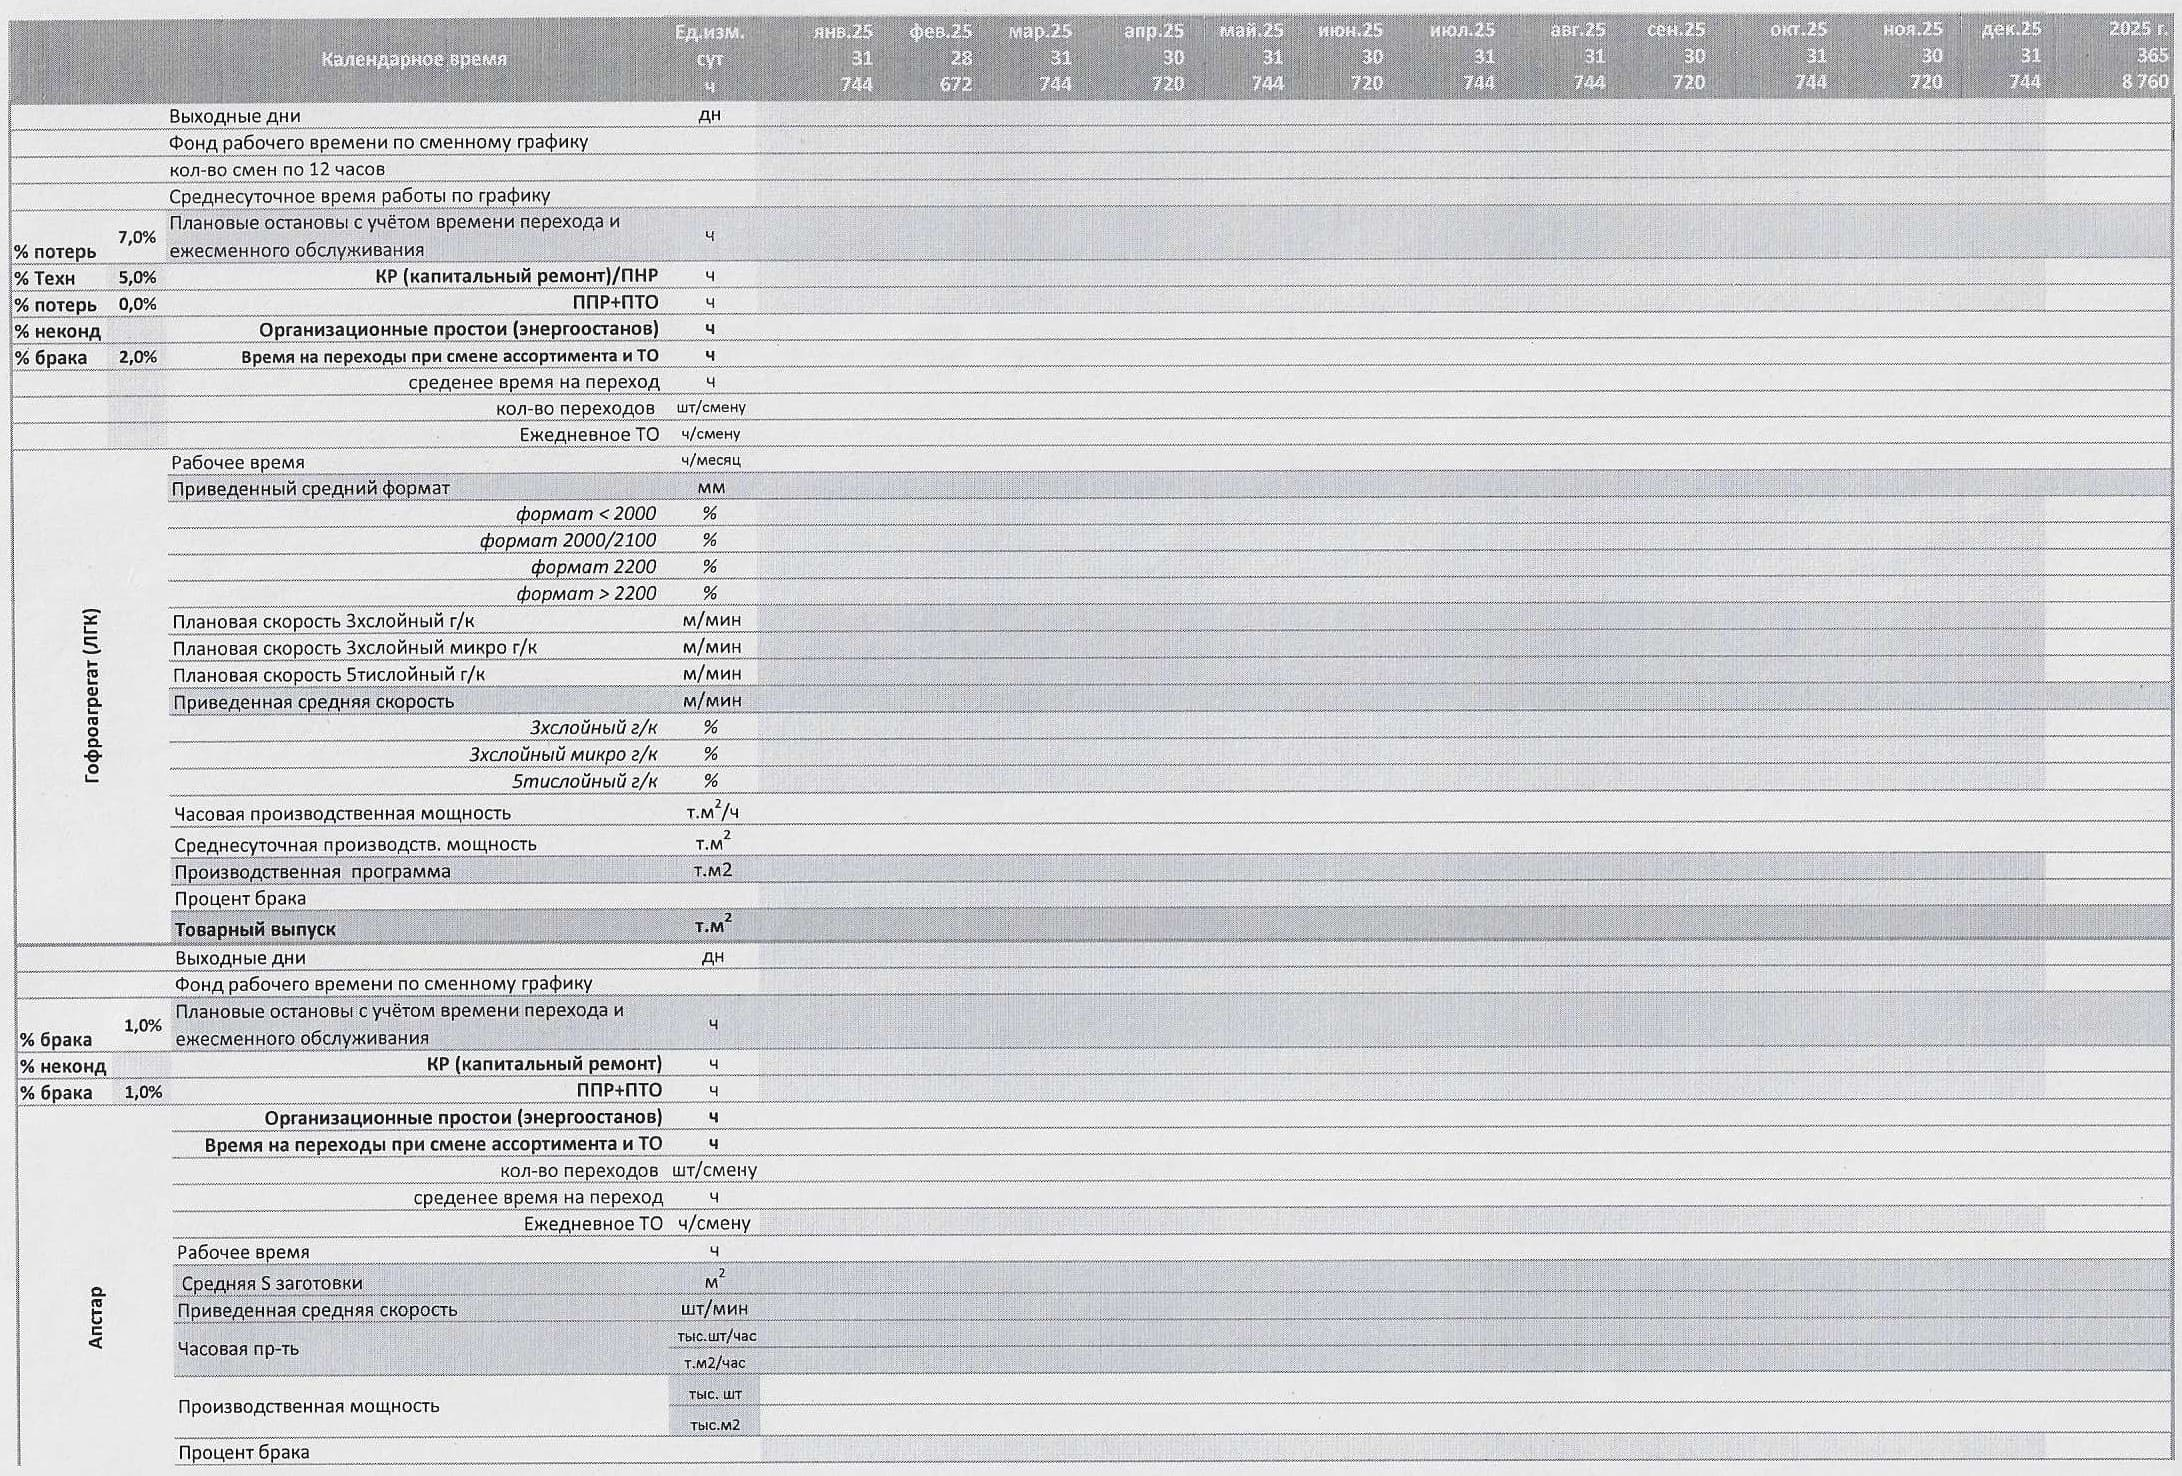
\includegraphics[height=0.6\textheight, width=1.3\textwidth, angle=90, keepaspectratio]{Pics/XI.1.jpg}
\end{center}
\caption{Форма ПРОФИНТЕХПЛАН}
\label{pic:XI.1}
\end{figure}
\clearpage

\begin{figure}
\begin{center}
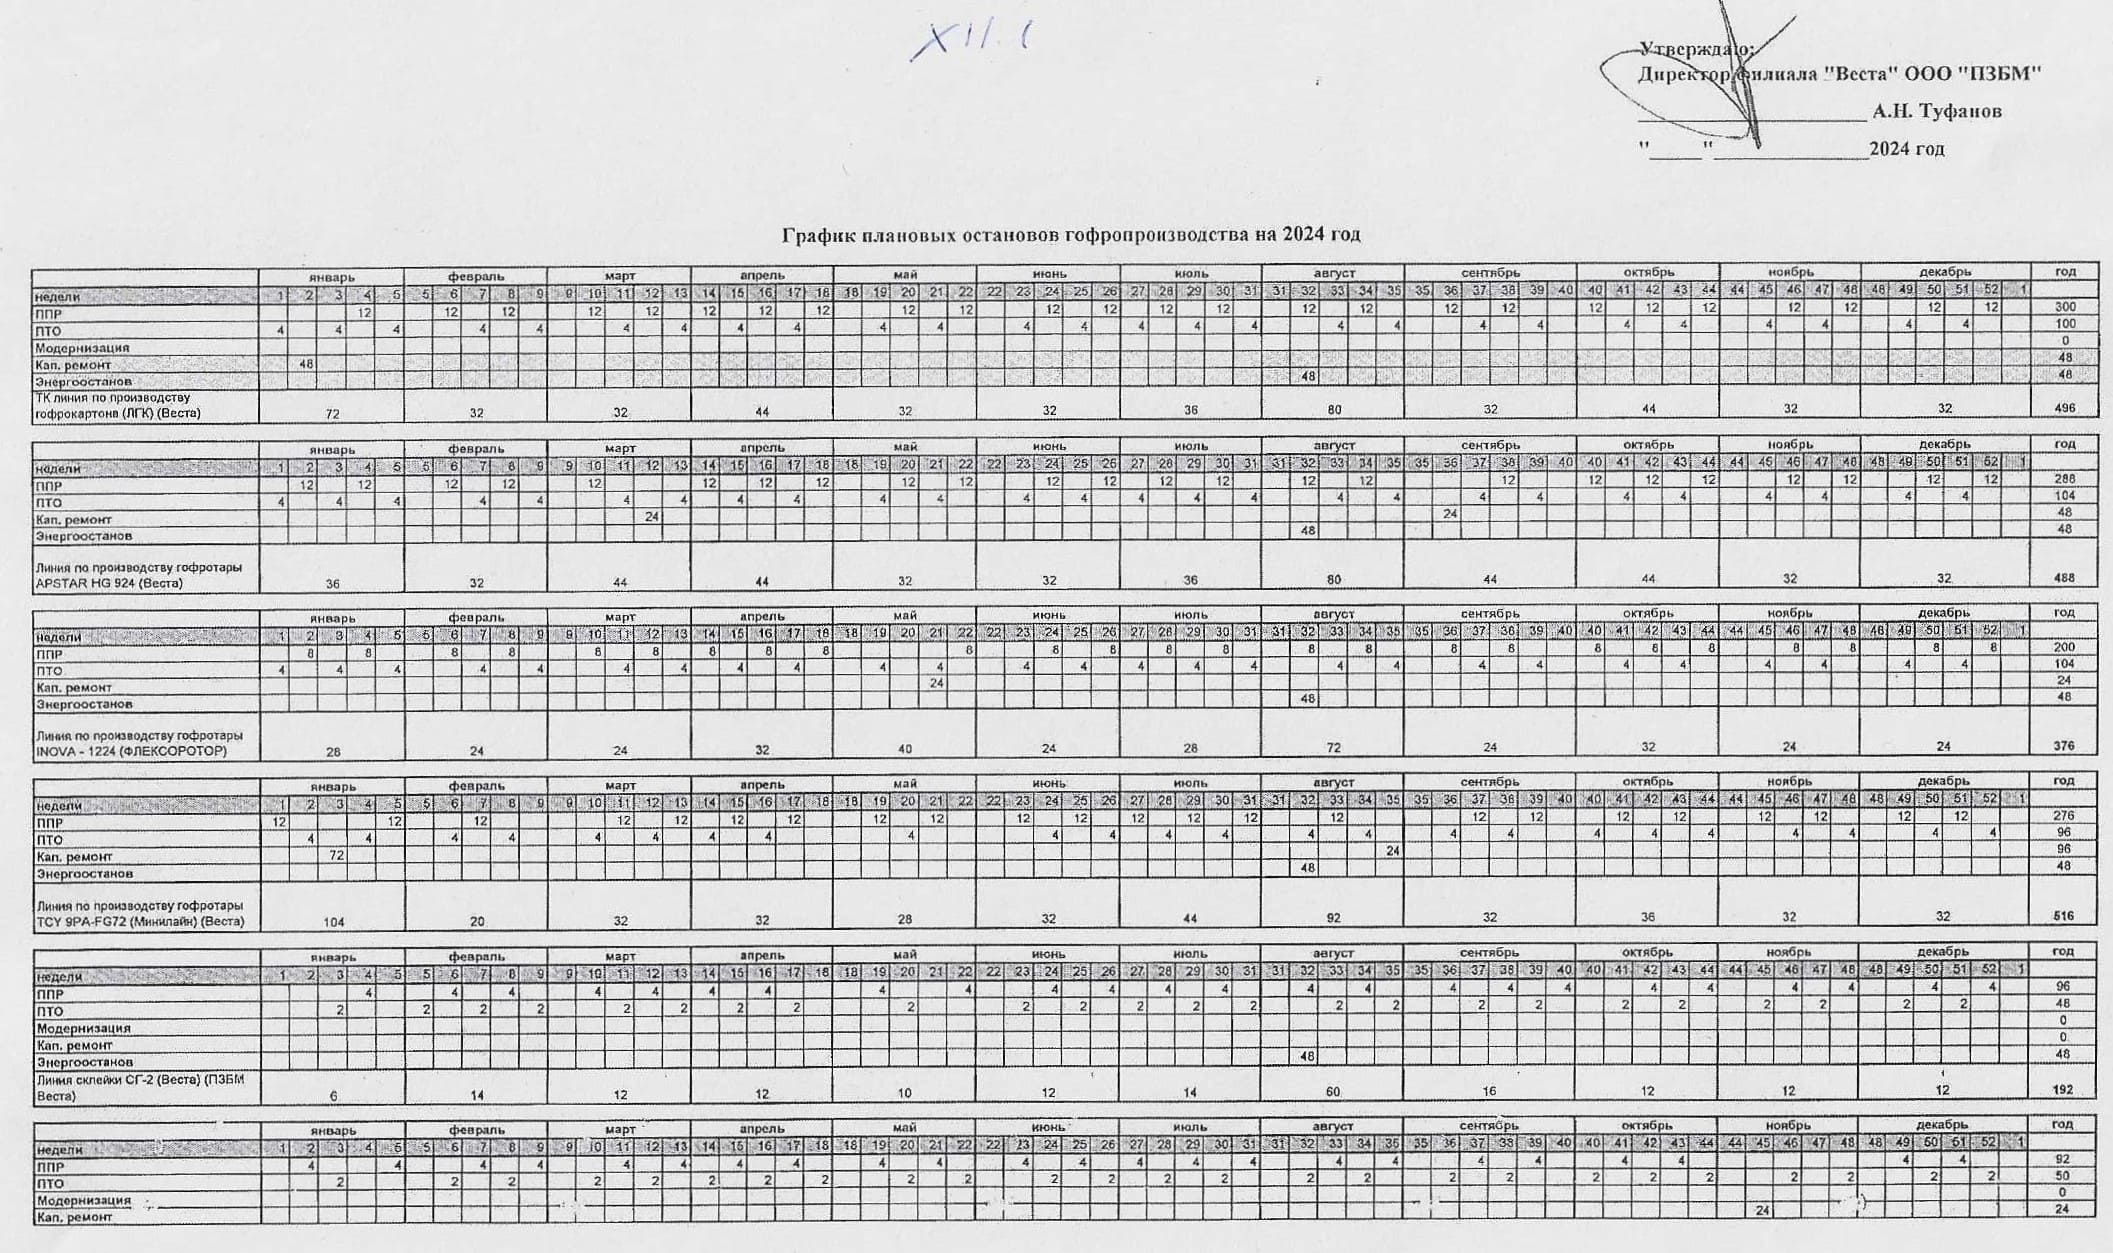
\includegraphics[height=0.6\textheight, width=1.3\textwidth, angle=90, keepaspectratio]{Pics/XII.1.jpg}
\end{center}
\caption{Годовой график плановых остановов}
\label{pic:XII.1.jpg}
\end{figure}
\clearpage

\begin{figure}
\begin{center}
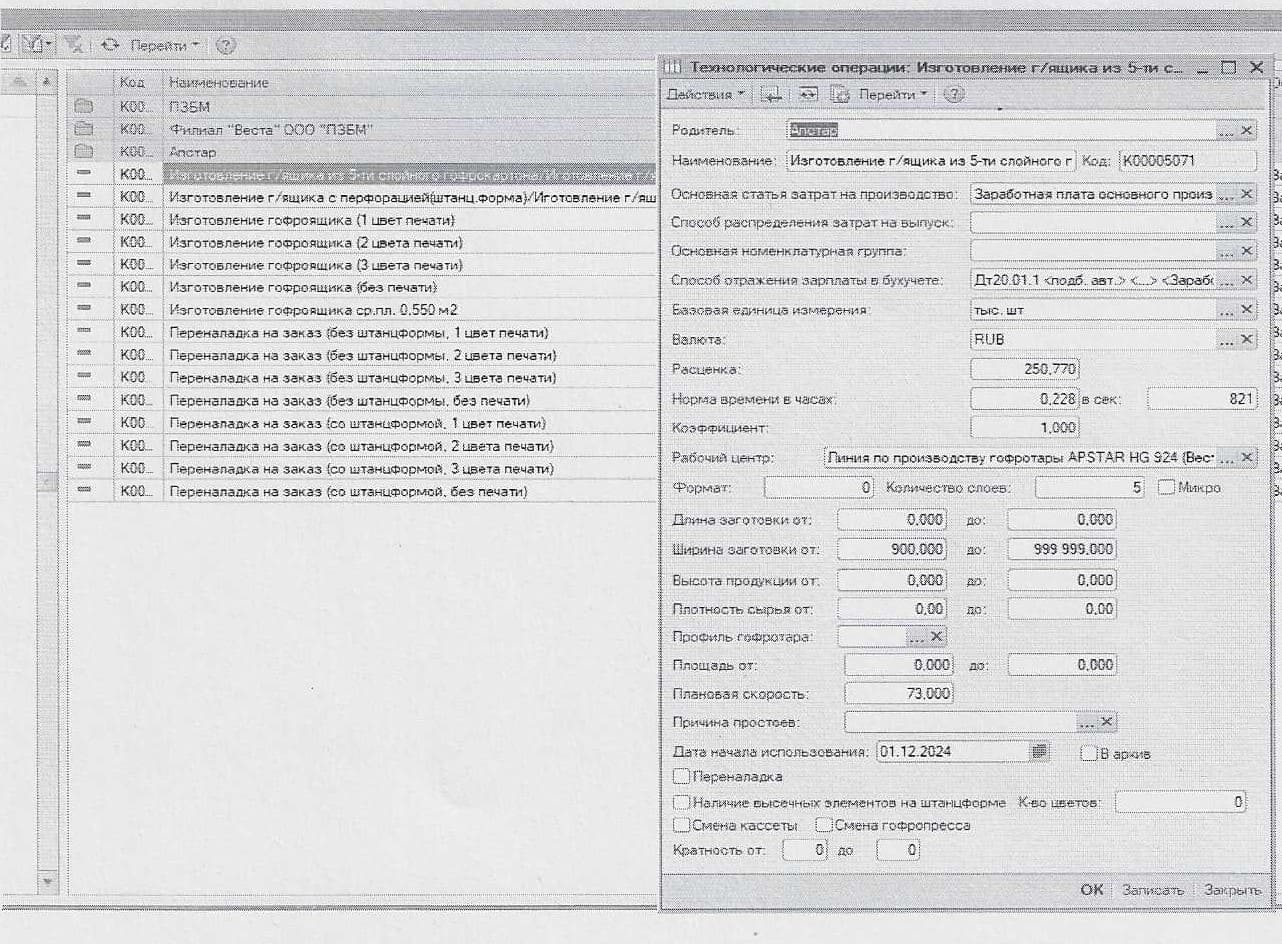
\includegraphics[height=0.6\textheight, width=1.3\textwidth, angle=90, keepaspectratio]{Pics/XI.12.jpg}
\end{center}
\caption{Нормирование времени и расценки в 1C:УПП}
\label{pic:XI.12.jpg}
\end{figure}
\clearpage

\begin{figure}
\begin{center}
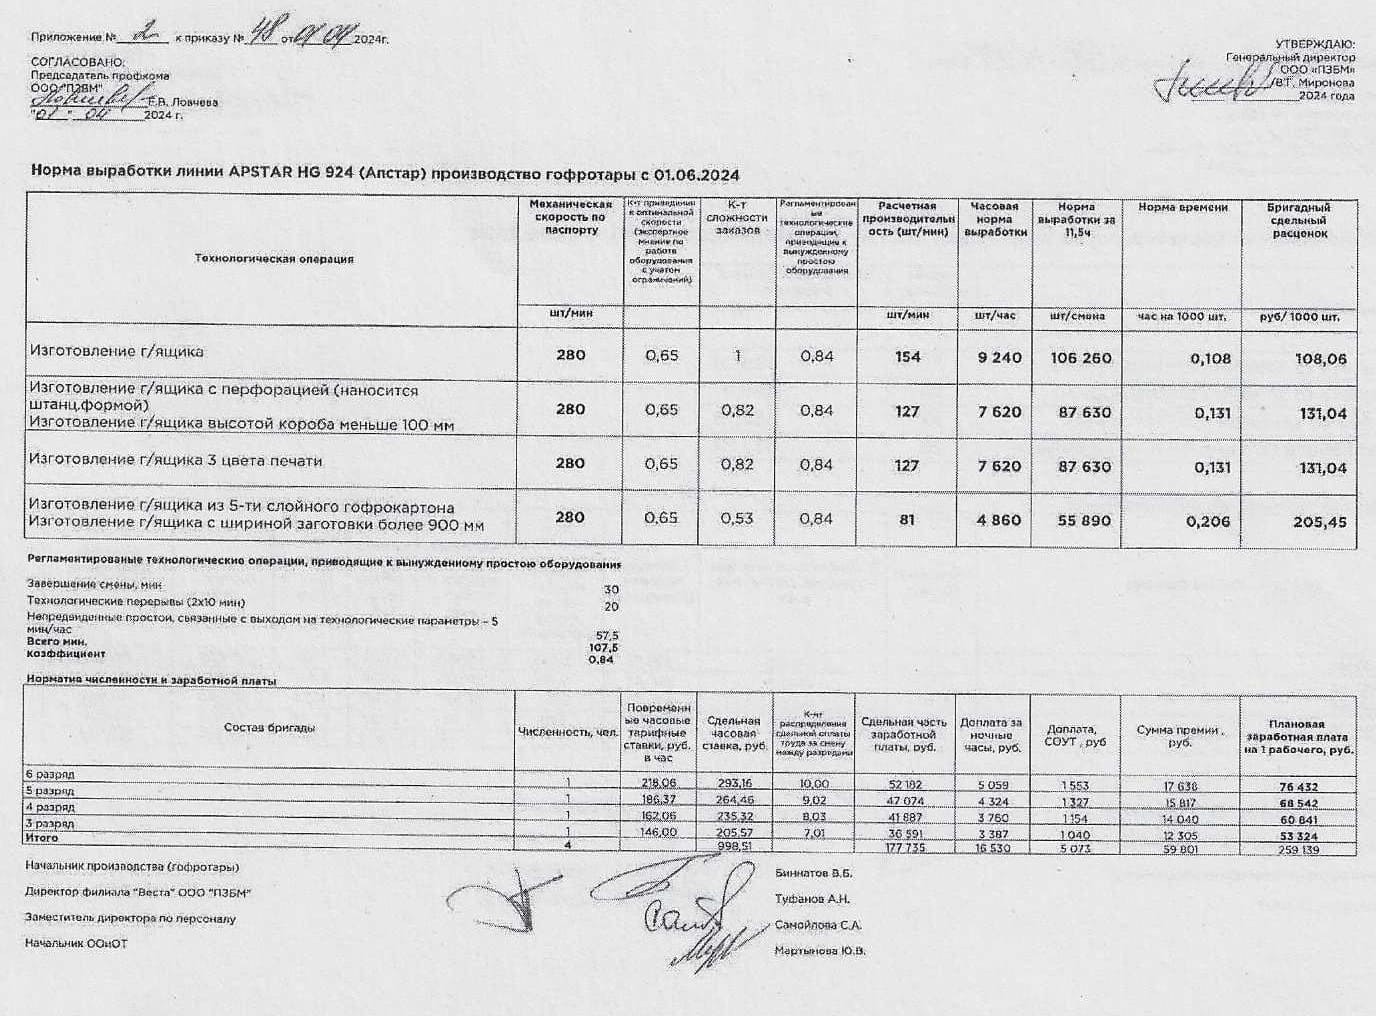
\includegraphics[height=0.6\textheight, width=1.3\textwidth, angle=90, keepaspectratio]{Pics/XI.11.jpg}
\end{center}
\caption{Утвержденная норма выработки на линию Апстар}
\label{pic:XI.11.jpg}
\end{figure}
\clearpage

\begin{figure}
\begin{center}
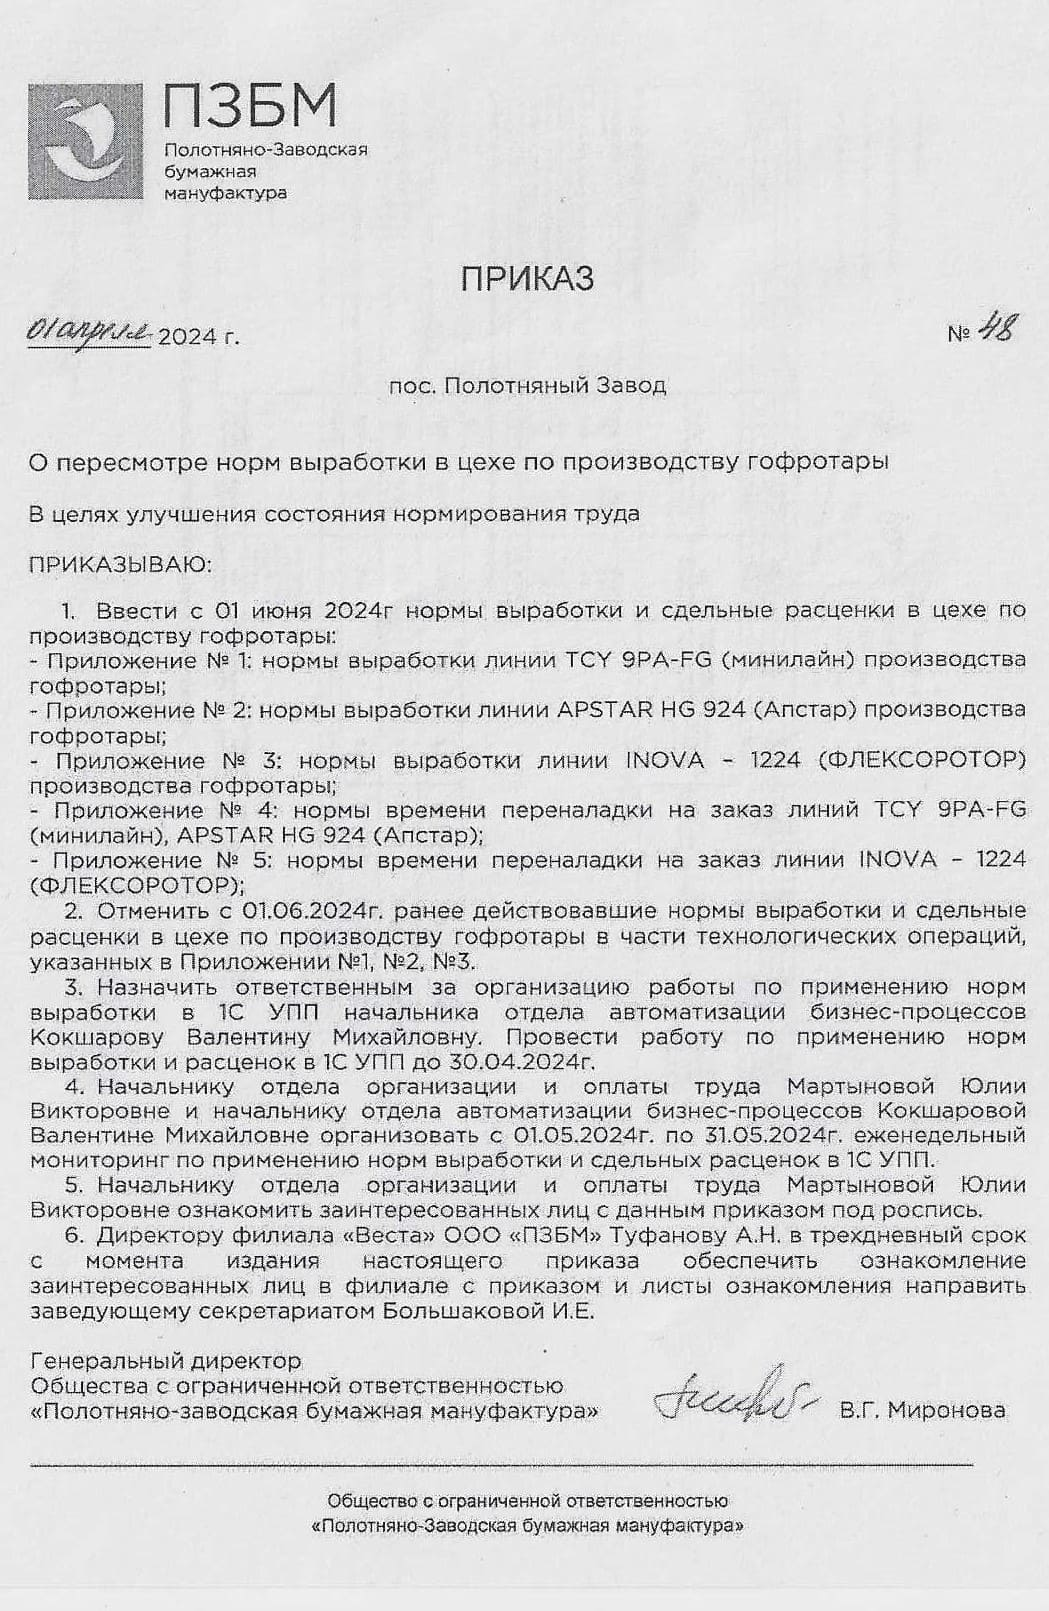
\includegraphics[height=0.8\textheight, width=1.5\textwidth, keepaspectratio]{Pics/XI.11..jpg}
\end{center}
\caption{Приказ о пересмотре норм выработки}
\label{pic:XI.11..jpg}
\end{figure}
\clearpage

\begin{figure}
\begin{center}
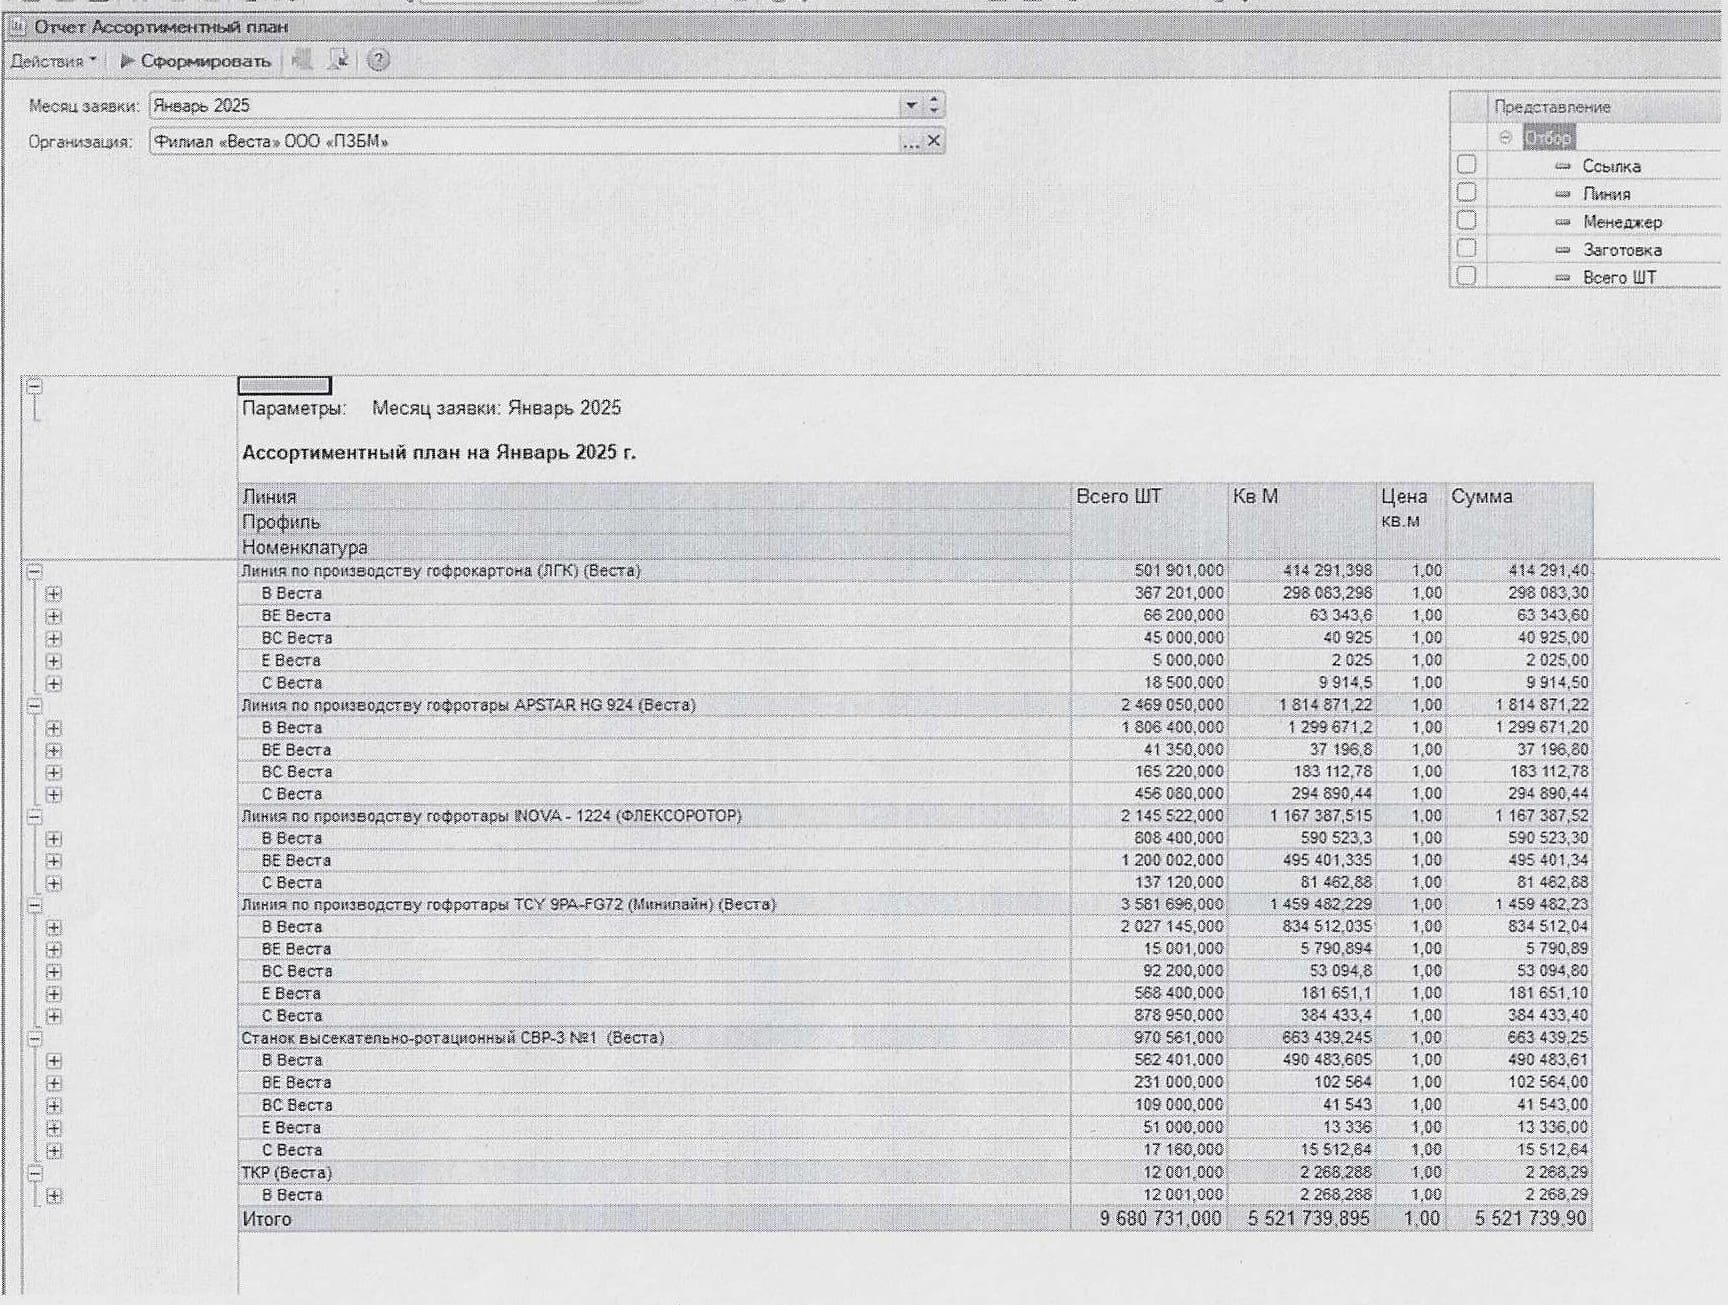
\includegraphics[height=0.5\textheight, width=1.3\textwidth, keepaspectratio]{Pics/I.5.6..jpg}
\end{center}
\caption{Форма Ассортиментный план}
\label{pic:I.5.6..jpg}
\end{figure}
\clearpage

\begin{figure}
\begin{center}
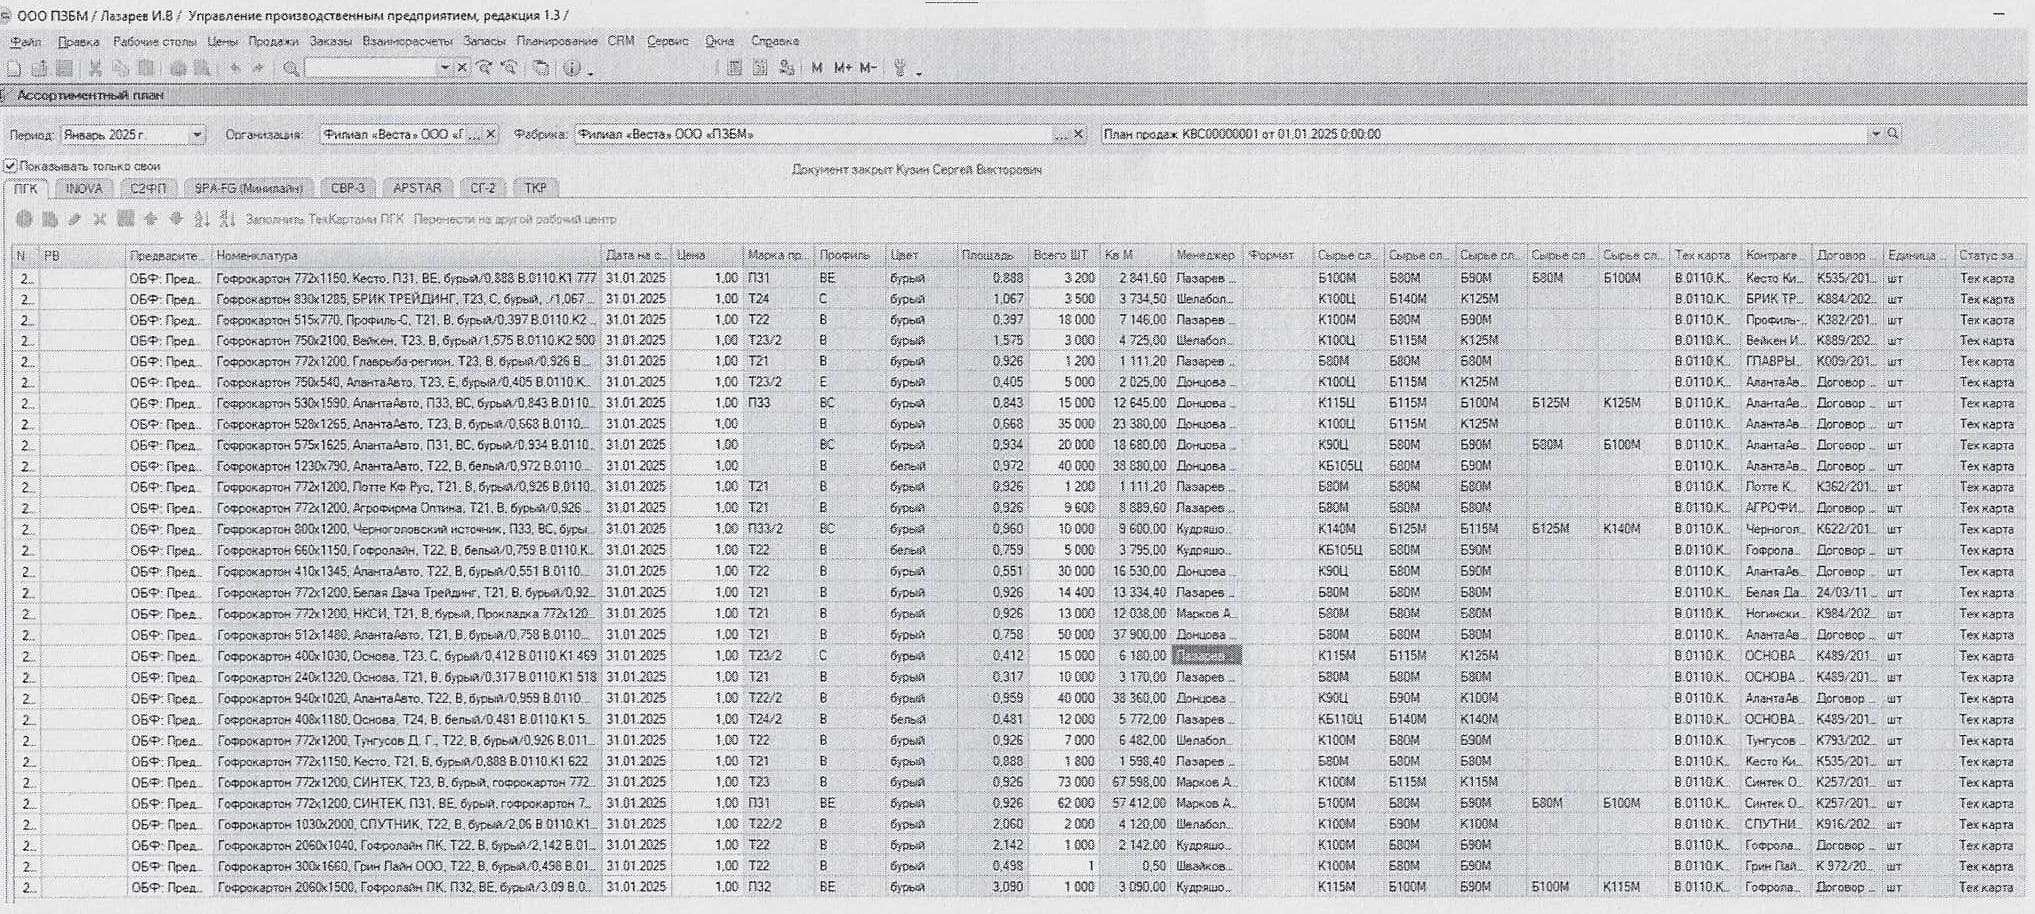
\includegraphics[height=0.3\textheight, width=1.3\textwidth, angle=90, keepaspectratio]{Pics/I.5.6.jpg}
\end{center}
\caption{Расширенная Форма Ассортиментный план}
\label{pic:I.5.6.jpg}
\end{figure}
\clearpage

%\ifx \notincludehead\undefined
\normalsize
\end{document}
\fi